\documentclass[12pt,reqno]{amsart}
\usepackage[margin=3cm]{geometry}

\usepackage{amsmath, amssymb, amsfonts, tikz, enumerate, graphicx, textcomp, caption, wrapfig, amsthm, todonotes, verbatim, cleveref, caption, float, mathabx, url}
\usetikzlibrary{calc, arrows}
\usepackage[procnames]{listings}
\usepackage{color, subfig}
\usepackage[section]{placeins}



\usepackage{color}
\definecolor{purple}{rgb}{0.5,0,1}

\newenvironment{dami}{
  \medskip
\begin{color}{blue}
    \textcolor{purple}{\textbf{Dami:}} 
}{
\end{color}
  \medskip
}


\newenvironment{cat}{
  \medskip
\begin{color}{red}
    \textcolor{red}{\textbf{Catherine:}} 
}{
\end{color}
  \medskip
}

\definecolor{keywords}{RGB}{255,0,90}
\definecolor{comments}{RGB}{0,0,113}
\definecolor{red}{RGB}{160,0,0}
\definecolor{green}{RGB}{0,150,0}
\lstdefinelanguage{Magma}%
  {%
   otherkeywords={:=,+:=,-:=,*:=},%
          % functions
   procnamekeys={function,func,intrinsic,procedure,proc},%
         % Booleans
   morekeywords={true,false},%
          % relations
   morekeywords=[2]{adj,and,cat,cmpeq,cmpne,diff,div,eq,ge,gt,in,is,join,le,lt,%
          meet,mod,ne,notadj,notin,notsubset,or,sdiff,subset,xor},%
          % keywords
   morekeywords=[3]{assigned,break,by,case,catch,continue,declare,default,%
          delete,do,elif,else,end,eval,exists,exit,for,forall,fprintf,if,local,%
          not,print,printf,quit,random,read,readi,repeat,restore,save,select,%
          then,time,to,try,until,vprint,vprintf,vtime,when,where,while},%
          % directives
   morekeywords=[4]{clear,forward,freeze,iload,import,load},%
          % error checks
   morekeywords=[5]{assert,assert2,assert3,error,require,requirege,requirerange},%
          % constructors
   morekeywords=[6]{car,comp,cop,elt,ext,frac,hom,ideal,iso,lideal,loc,map,%
          ncl,pmap,quo,rec,recformat,rep,rideal,sub},%
          % other constructors (semi-reserved)
   morekeywords=[7]{AbelianGroup,AdditiveCode,AffineAlgebra,Algebra,%
          AssociativeAlgebra,Character,CliffordAlgebra,Design,Digraph,%
          ExtensionField,FPAlgebra,FiniteAffinePlane,FiniteProjectivePlane,%
          Graph,Group,GroupAlgebra,IncidenceStructure,LieAlgebra,LinearCode,%
          LinearSpace,MatrixAlgebra,MatrixGroup,MatrixRing,Monoid,%
          MultiDigraph,MultiGraph,NearLinearSpace,Network,PartialMap,%
          PermutationGroup,PolycyclicGroup,QuaternionAlgebra,Semigroup,%
          ZModule},%
          % functions
   morekeywords={[8]function,func,intrinsic,procedure,proc,return},%
      sensitive,%
      morecomment=[l]//,%
      morecomment=[s]{/*}{*/},%
      morecomment=[s]{\{}{\}},%
      morestring=[b]"%
  }[keywords,procnames,comments,strings]%
\lstset{language=Python, 
        basicstyle=\ttfamily\small, 
        keywordstyle=\color{keywords},
        commentstyle=\color{comments},
        stringstyle=\color{red},
        breaklines=true,
        showstringspaces=false,
        identifierstyle=\color{green},
        procnamekeys={def,class}}
%\usepackage[T1]{fontenc}
%\usepackage[urw-garamond]{mathdesign}
\usepackage{tikz-cd}\tikzset{node distance=2cm, auto}
\DeclareMathOperator{\Aut}{Aut}
\DeclareMathOperator{\Hom}{Hom}
\DeclareMathOperator{\Jac}{Jac}
\DeclareMathOperator{\Sym}{Sym}
\DeclareMathOperator{\Alt}{Alt}
\DeclareMathOperator{\Corr}{Corr}
\DeclareMathOperator{\im}{im}
\DeclareMathOperator{\uncurry}{uncurry}
\DeclareMathOperator{\Pic}{Pic}
\DeclareMathOperator{\Div}{Div}
\newcommand{\C}{\mathbb{C}}
\newcommand{\Z}{\mathbb{Z}}
\newcommand{\F}{\mathbb{F}}
\newcommand{\G}{\mathbb{G}}
\newcommand{\Q}{\mathbb{Q}}
\newcommand{\R}{\mathbb{R}}
\newcommand{\n}{\newline}
\newcommand{\mc}{\mathcal}
\newcommand{\te}{\text}
\newcommand{\bb}{\mathbb}
\renewcommand{\P}{\mathbb{P}}
\newcommand{\BBF}{\overline{\F_p}}
\newcommand\mapsfrom{\mathrel{\reflectbox{\ensuremath{\mapsto}}}}
\definecolor{codegray}{gray}{0.9}
\newcommand{\code}[1]{\colorbox{codegray}{\texttt{#1}}}
\newtheorem{theorem}{Theorem}
\newtheorem*{thm*}{Theorem}
\newtheorem*{proposition}{Proposition}
\newtheorem{lemma}[theorem]{Lemma}
\newtheorem*{lemma*}{Lemma}
\newtheorem*{qlemma*}{``Lemma"}
\newtheorem{cor}[theorem]{Corollary}
\newtheorem{conjecture}[theorem]{Conjecture}
\newtheorem{postulate}[theorem]{Postulate}
\newtheorem*{question}{Question}
\theoremstyle{definition}
\newtheorem{defn}{Definition}
\newtheorem{example}[theorem]{Example}
\theoremstyle{remark}
\newtheorem*{remark}{Remark}
\newtheorem*{notation}{Notation}
\newtheorem*{note}{Note}
\newcommand{\sss}{\ss$\text{ }$}
\newcommand{\ti}{\todo[inline]}
\newcommand{\DD}{\Delta\kern -8.3pt {\diamond} \kern -4.5pt \cdot \:}
\newenvironment{myproof}[1][``\proofname '']{%
  \proof[ #1]%
}{\endproof}




\title{Exhibiting Automorphism Groups via Tessellations} 
\author{Dami Lee and Catherine Ray}

\begin{document}

	
\maketitle

\begin{abstract}
Given a curve with cone metrics, we introduce a new conjectural method for computing its automorphism group by constructing a hyperbolic tessellation that exhibits the automorphism group of the curve. The curves of our interest are cyclic covers over the Riemann sphere, as we can pin down explicit cone metrics on such curves. Given a cone metric, we locate all Weierstrass points on the curve, with which we construct a tessellation. We calculate the automorphism group of the tessellation combinatorially, and conjecture that it is isomorphic to the automorphism group of the curve. Examples we explore include Klein's quartic and Fermat's quartic, where all Weierstrass points have the same weight, and also Schoen's I-WP minimal surface, where the Weierstrass points have different weights. We verify this conjecture in several key examples with programs based on the algorithms of Bruin-Sijsling-Zotine.
\end{abstract}



\section{Introduction}


In \cite{dami}, the first author studies the underlying curve of an embedded triply periodic polyhedral surface $\Pi \subset \R^3$ equipped with a polyhedral cone metric. By triply periodic, we mean that $\Pi$ is invariant under a rank-three lattice $\Lambda \subset \R^3$ by translations. The polyhedral surface is tiled by triangles with eight meeting at each vertex. With identifications, the underlying curve $C = \Pi / \Lambda$ is a closed genus three curve and with the induced polyhedral cone metric, it is invariant under an order-eight rotation. This order-eight symmetry is not visible on the embedding of the polyhedral surface $\Pi \subset \R^3.$ The quotient under the $\Z/ 8 \Z$-action on $C$ yields the Riemann sphere where the cover is branched over three points. We say that a curve $C$ is a $d$-fold cyclic cover branched over a sphere if $C / (\Z / d \Z) = \mathbb{C}\mathbb{P}^1$ for some positive integer $d.$ A cyclic cover over a sphere gives rise to various cone metrics with which one can compute a basis of holomorphic 1-forms on $C.$ With explicit cone metrics and symmetries induced from the polyhedral surface, the author locates all Weierstrass points on $C.$ Then by finding a hyperbolic tessellation $\Delta$ on the curve where all vertices are Weierstrass points, the author computes $\Aut(\Delta)$ and shows that $\Aut(\Delta) \simeq \Aut(C)$. We note that the hyperbolic tessellation coincidentally corresponds to the euclidean tiling on $\Pi.$ [[the author computes the automorphism group of the tessellation that acts freely and transitively on the tiles]]. We call a tessellation with this property \textbf{all-seeing}. This all-seeing tessellation provides a concrete way of presenting the automorphism group of a curve, as opposed to presenting the automorphism group as an action on the coefficients of a polynomial describing the curve (appendix A, \cite{silverman}). % the bit on Fermat is moved to a later section

Although we do not prove any theorem in this paper, we conjecture that given a cyclic cover branched over $\mathbb{C}\mathbb{P}^1,$ there exists a tessellation that exhibits the automorphism group of the curve. Further, we present an algorithm to construct this tessellation. We heavily rely on the first author's thesis \cite{dthesis} where they discuss cone metrics on cyclic covers over $\mathbb{C}\mathbb{P}^1$ and classify all of them up to genus five. We summarize in section~\ref{sec: dthesis} how to find cone metrics, find a basis of holomorphic 1-forms, find a plane curve model, and locate Weierstrass points given only a construction of a cyclic cover over a sphere. Furthermore, from cone metrics we can compute period matrices, which we use in a sequel to this paper. 

This project began from the second author wondering if the first author's method for computing the automorphism group could be applied in more generality to exhibit the automorphism group of any principally-polarized Jacobian variety. As Torelli's theorem gives the relation between the automorphism group of a genus $g$ curve $C_g$ and its Jacobian variety $\Jac(C_g$, the aim was to find a combinatorial way to exhibit the automorphisms of the Jacobian via an all-seeing tessellation. The initial naive approach was finding an all-seeing tessellation of the Jacobian by taking the image of an all-seeing tessellation of $C$ under one of two maps: either an Abel-Jacobi map $C_g \hookrightarrow \Jac(C_g)$, or embedding the $g$-th symmetric product of the tessellation on $C_g \hookrightarrow \Sym^g(C_g) \to \Jac(C_g)$, where the second map is a birational equivalence. We found that it is computationally easier to find the all-seeing tessellation on the underlying curve and use the precise Torelli theorem to get a concrete presentation of the automorphism group of its principally-polarized Jacobian. We thus focus on formulating the all-seeing tessellation in more generality.

In this paper, we conjecturally extend the first author's all-seeing method to curves that have Weierstrass points of different weights. In section~\ref{sec: dthesis}, we discuss how examples that naturally yield cone metrics appear in the wild, that is, cyclic covers that are branched over $\mathbb{C}\mathbb{P}^1.$ Then given a cone metric, we discuss how to achieve plane curve models and find Weierstrass points. In section~\ref{sec:flagflag}, we show an algorithm that yields a tessellation given only the construction of a cyclic cover over $\mathbb{C}\mathbb{P}^1.$ Then we compute the automorphism group of this tessellation. We conjecture that the automorphism group of this tessellation is the same as the automorphism group of the original curve which we compute by already known methods. In section~\ref{sec:examples}, we verify this conjecture for examples of cyclic covers over $\mathbb{C}\mathbb{P}^1.$ Independently, we will compute the automorphism group of the curves using a program based on the algorithm of Bruin-Sijsling-Zotine \cite{jeroen}. This program requires only the plane curve model which we obtain from cone metrics. 

This paper proves no theorems, but rather demonstrates the strength and potential of a computational technique, and a new way to present the automorphisms of a curve and its Jacobian.

\section*{Acknowledgements} 
The first author would like to thank Matthias Weber for his guidance at the beginning of this project. The second author would like to thank Magma and Sage contributors Edgar Costa, John Voight, Nicolas Mascot, and above all Jeroen Sijsling, who generously offered incredibly detailed and consistent help in computing the automorphism groups of Jacobians. This material is based upon work supported by the National Science Foundation under Grant No. DMS-1440140 while the first author was in residence at the Mathematical Sciences Research Institute in Berkeley, California, during the Fall 2019 semester. The second author is partially supported the National Science Foundation GRFP under Grant Number DGE 1842165. 

\section{Background}
\label{sec: dthesis}
In \cite{dami}, the first author investigates a triply periodic polyhedral surface $\Pi$ embedded in $\mathbb{R}^3.$ By triply periodic, we mean that $\Pi$ is invariant under a rank-three lattice $\Lambda \subset \R^3.$ We take its fundamental piece $C = \Pi / \Lambda$ and by appropriate identification, we get a genus three curve where we pin down the conformal structure by descending the polyhedral cone metric to its quotient. Although it is not visible on the embedded surface, $C$ is intrinsically invariant under an order-eight rotational symmetry, and its quotient under $\Z/ 8 \Z$ yields $\mathbb{C}\mathbb{P}^1.$ We focus on curves that are cyclic covers over $\mathbb{C}\mathbb{P}^1,$ hence we will devote this section to providing the background. This section is a summary of chapter 3 from the first author's thesis \cite{dthesis}. 

\subsection{Cone metrics}
First, we discuss the topological construction of cyclic covers over $\mathbb{C}\mathbb{P}^1.$ This will naturally yield cone metrics on the curves.

\subsubsection*{Construction of cyclic covers over $\mathbb{C}\mathbb{P}^1$}
\begin{defn} A curve $C$ is a $d$-fold cyclic cover over $\mathbb{C}\mathbb{P}^1$ if $C / (\Z/ d \Z) = \mathbb{C}\mathbb{P}^1.$ \end{defn}

We construct such a curve in the following way: for $n$ distinct points $p_i, \ldots , p_n \in \mathbb{C}\mathbb{P}^1,$ let $Y := \mathbb{C}\mathbb{P}^1 \backslash \{p_1, \ldots, p_n\}$ and let $\gamma_i$ be a branch cut from $p_i$ to some $q \in Y$ so that $\gamma_i$ are mutually disjoint. To each $i,$ we assign a positive integer $d_i$ and call it the \textbf{branching index}. Let $d$ be the degree of the covering map and use $j$ to label $Y_1, \ldots , Y_d.$ For each $i$ and $j,$ we identify the ``left side'' of $\gamma_i$ of $Y_j$ to the ``right side'' of $\gamma_i$ of $Y_{j + d_i \pmod d}.$ We denote such a covering $C$ by a $d$-tuple $d (d_1, \ldots , d_n).$


\begin{remark} Given a $d$-fold cyclic cover over $Y$ with branching indices $(d_1, \ldots , d_n),$ a covering is uniquely defined up to homeomorphism. That is, the construction only depends on $d_i$ and is independent of $p_i,$ $\gamma_i,$ and $q.$ The covering is closed if and only if $\sum\limits_{i=1}^n d_i \equiv 0 \pmod d,$ and is connected if and only if $\gcd (d_1, \ldots, d_n) = 1.$ We assume these two conditions. Then the genus of the curve $g(C) = \frac{d (n-2)}{2} + 1 - \frac{1}{2} \sum\limits_{i=1}^n \gcd(d,d_i)$ follows from Riemann-Hurwitz formula. 
\end{remark}

\subsubsection*{Branching indices on Octa-4}
As a running example, we will look at the curve from \cite{dami}. It is there called Octa-4 due to the formation of $\Pi.$ The underlying genus three curve $C = \Pi / \Lambda$ (Figure~\ref{fig:125} (reprinted from \cite{dami})) is invariant under an order-eight rotational symmetry. The curve is an eightfold cyclic cover over $\mathbb{C}\mathbb{P}^1$ denoted as $8 (1, 2, 5).$

\begin{figure}[htbp] %  figure placement: here, top, bottom, or page
   \centering
   \includegraphics[width=2in]{figures/125_base_.pdf} 
	\caption{Hyperbolic tessellation on $8(1, 2, 5)$}
	\label{fig:125}
\end{figure}

The euclidean triangles on the fundamental piece of $\Pi$ have a one-to-one correspondence to the hyperbolic triangles.

For each $i,$ there are $\gcd(d, d_i)$ preimages $\widetilde{p_i}$ of $p_i$ on $C.$ Hence, each $\widetilde{p_i}$ is a cone point. To pin down a flat metric on $C,$ that is, a holomorphic 1-form on $C,$ we pull back a cone metric from $\mathbb{C}\mathbb{P}^1.$ We say that a cone metric on $\mathbb{C}\mathbb{P}^1$ is \textbf{admissible} if its pullback yields a flat structure on $C.$ The following proposition is a version of Gauss-Bonnet theorem.

\begin{proposition} Given a compact Riemann surface of genus $g$ with a cone metric, let $p_1, \ldots, p_n$ be distinguished points with respective cone angles $\theta_i.$ Then $\sum\limits_{i=1}^n \theta_i = 2 \pi (2 g - 2 + n).$
\end{proposition}

\begin{figure}[htbp] %  figure placement: here, top, bottom, or page
   \centering
   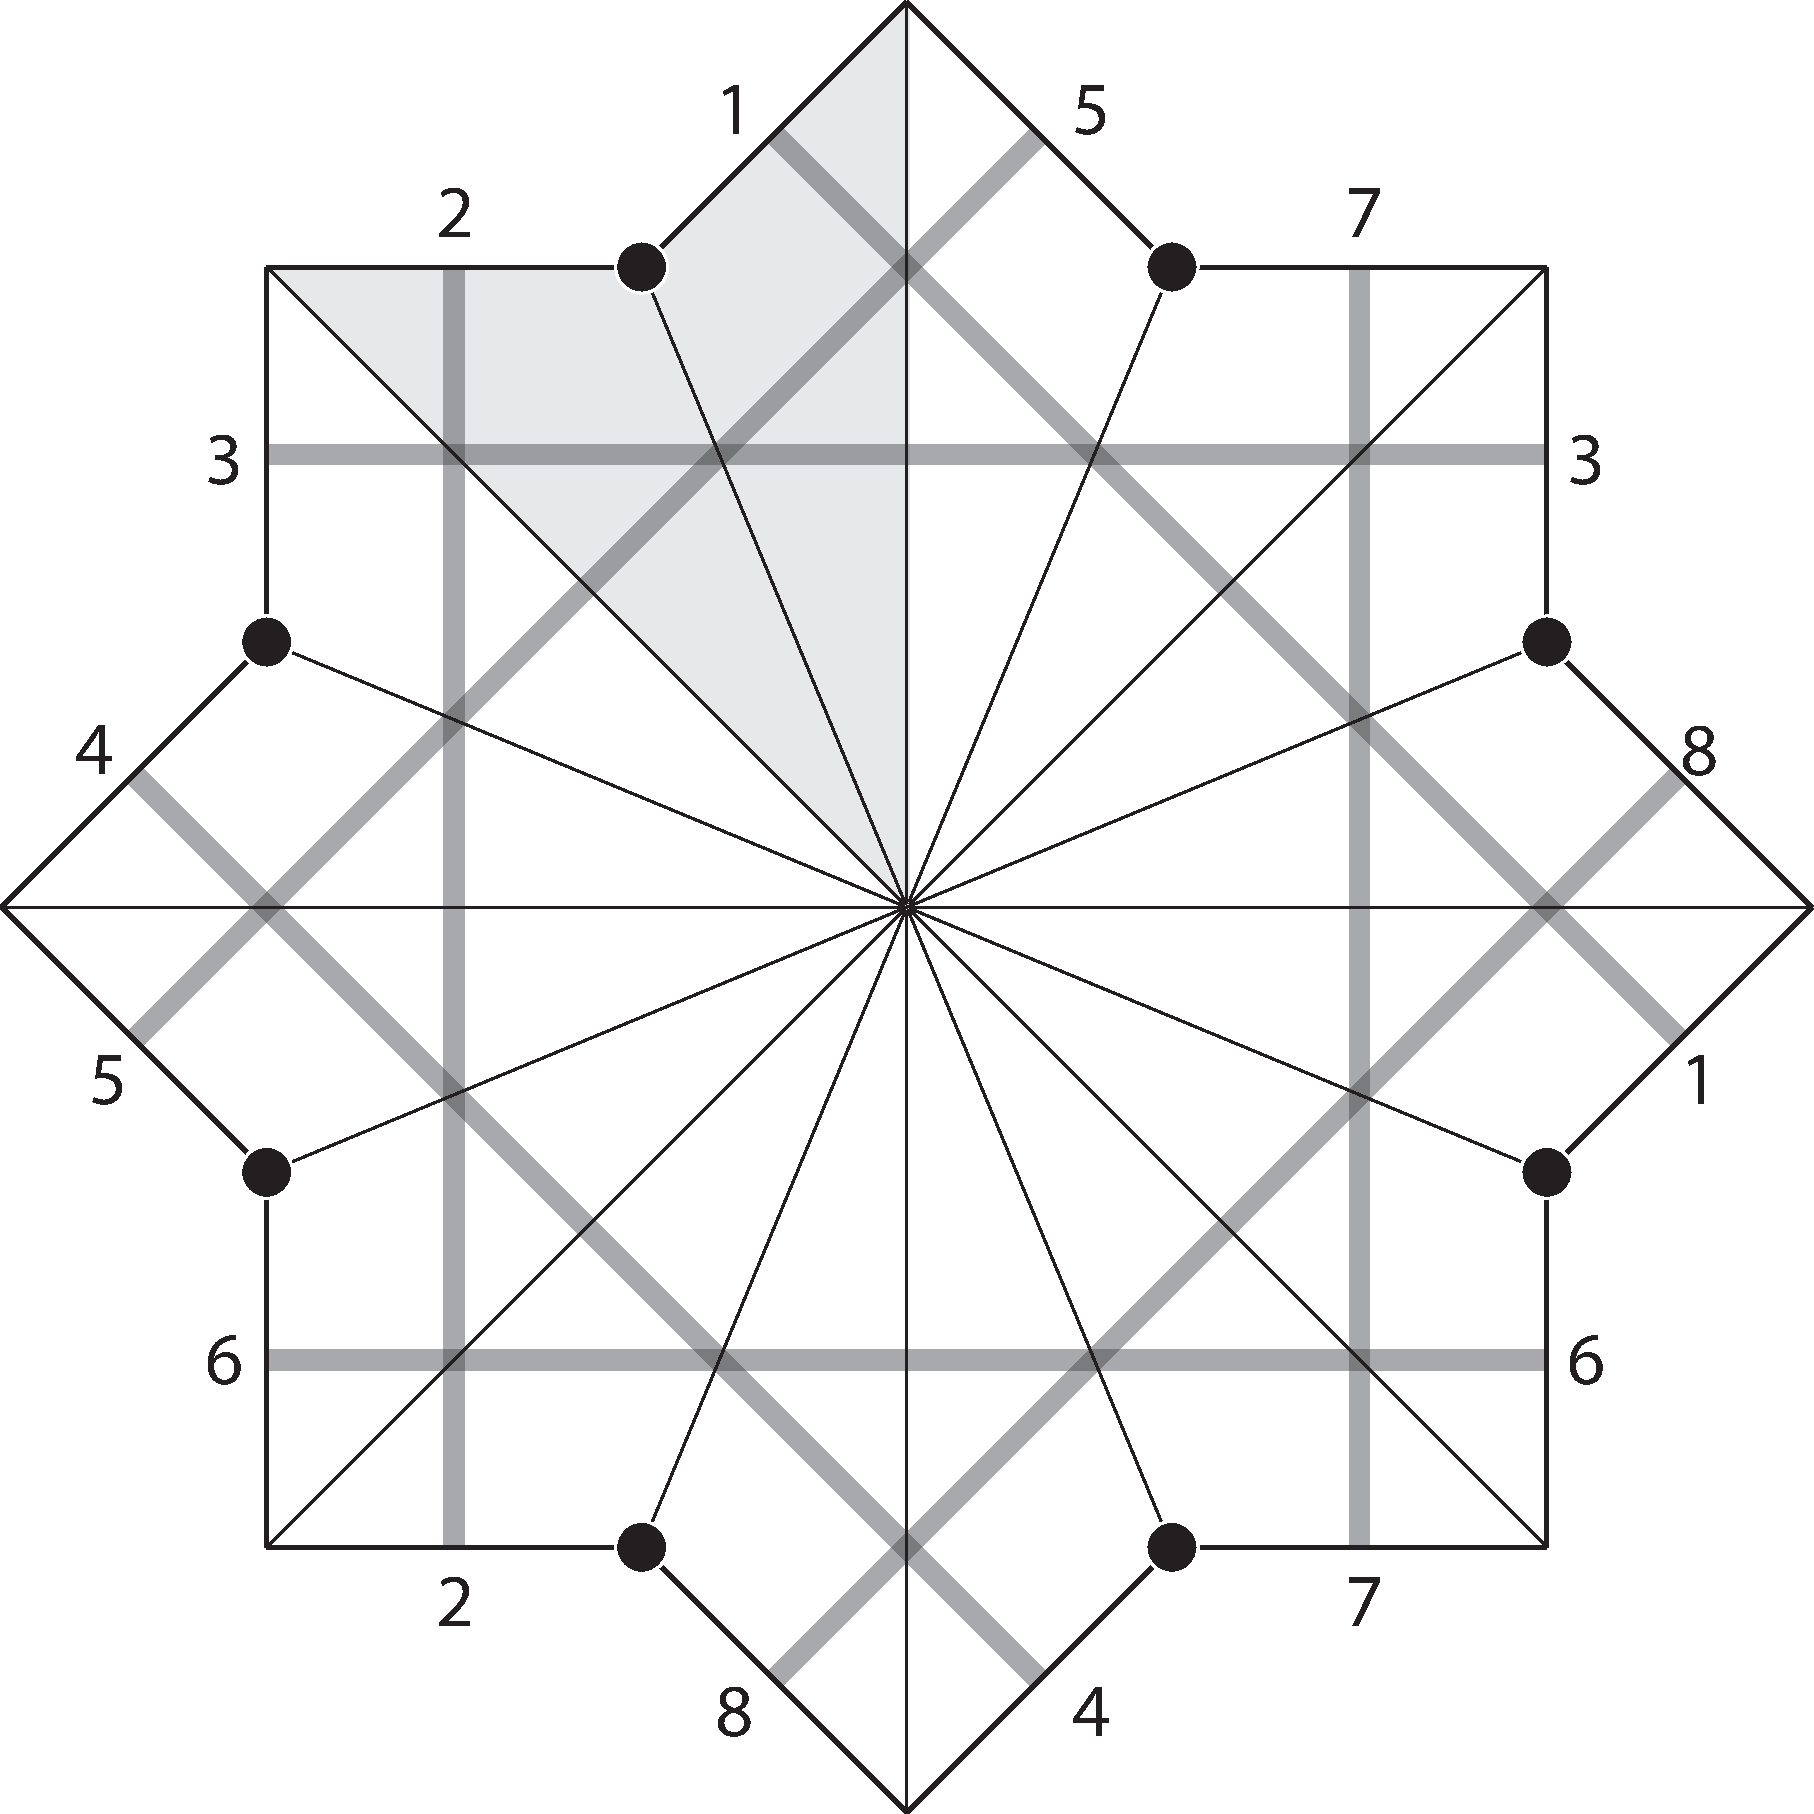
\includegraphics[width=2in]{figures/125_flat.pdf} 
	\caption{A flat metric on $8(1, 2, 5)$}
	\label{fig:125_flat}
\end{figure}

In other words, the sum of cone angles on a genus zero curve is $2 \pi (n - 2).$ Given branching indices such that $\sum\limits_{i=1}^n d_i = d (n - 2),$ we get a cone metric on the Riemann sphere with cone angles $\frac{2 \pi d_i}{d}$ at each $p_i.$ For example, by putting a cone metric on the quotient sphere where the cone angles are $\frac{1 \pi}{4}, \frac{2 \pi}{4},$ and $\frac{5 \pi}{4}$ as in Figure~\ref{fig:125_flat}, one can see that the identification of edges are by translations. In other words, there is a flat metric on the eightfold cover of the sphere. 

Our goal is to find other cone metrics that realize the same underlying curve. If $\sum\limits_{i=1}^n d_i \neq d (n - 2),$ then we modify the cone angles by $\frac{2 \pi a_i}{d}$ so that where $a_i \equiv d_i \pmod d$ for each $i.$ As each cone metric corresponds to a holomorphic 1-form, we use the following notion of multipliers that give rise to other cone metrics in order to get a basis of 1-forms.

\begin{defn} Given branching indices $d (d_1, \ldots , d_n),$ we say $a \in \{1, \ldots, d - 1\}$ is a \textbf{multiplier} if the cone metric given by cone angles $\frac{2 \pi}{d} (a \cdot d_1 \pmod d, \ldots , a \cdot d_n \pmod d)$ is admissible. 
\end{defn}

It is proved in \cite{dthesis} (Theorem 3.15) that for $n = 3,$ there are exactly $g$ multipliers. 

\subsubsection*{Admissible cone metrics on Octa-4} Given branching indices $8 (1, 2, 5),$ multipliers 1, 2, and 5 give rise to cone metrics with cone angles $\frac{2 \pi}{8}(1, 2, 5),$ $\frac{2 \pi}{8}(2, 4, 2),$ and $\frac{2 \pi}{8}(5, 2, 1),$ respectively. These cone metrics yield a basis of holomorphic 1-forms with the following divisors: $$(\omega_1) = 4 \widetilde{p_3}, \qquad (\omega_2) = \widetilde{p_1} + \widetilde{p_{2_1}} + \widetilde{p_{2_2}} + \widetilde{p_3}, \qquad (\omega_3) = 4 \widetilde{p_1}.$$

\begin{remark} Note that 3, 6, and 7 are not multipliers as their corresponding forms do not yield canonical divisors. On the other hand, 4 is not a multiplier as the cone metric derived from cone angles $\frac{2 \pi}{8} (4, 0, 4)$ is not admissible. This induces a meromorphic form whose divisor is $3 \widetilde{p_1} - \widetilde{p_2}_1 - \widetilde{p_2}_2 + 3 \widetilde{p_3}.$ \end{remark}

\subsection{Plane curve model}
\label{subsec:polynomial} Given brancing indices $d (d_i),$ we write $C$ as $y^d - (x - p_1)^{d_1} (x - p_2)^{d_1} \cdots (x - p_n)^{d_n}.$ In section~\ref{sec:examples}, we will show examples where the degree of the polynomial can be reduced and hence the polynomial is not uniquely defined. However, different polynomials representing the same curve yield the same output (automorphism group) when put in the program in \cite{jeroen}.


\subsubsection*{Plane curve model on Octa-4}
With branching indices $8 (1, 2, 5),$ the underlying curve of Octa-4 is written as $y^8 - x (x-1)^2.$ However, in Theorem 5.1 from \cite{dami} the author shows that it can also be written as $y^4 - x (x-1) (x+1)$ and shows that this is equivalent to Fermat's quartic.

\subsection{Weierstrass points and how to find them}

A Weierstrass point $p \in C$ is a point where there are functions on $C$ with unusual pole orders at $p$ and nowhere else. In other words, they are points where the dimension-count of the Riemann-Roch theorem is not generic. We say that a point is generic if it is not a Weierstrass point. Hurwitz showed that for $g \geq 2,$ there are finitely many Weierstrass points on $C$ and the number of Weierstrass points is bounded by $2 g + 1 \leq |W(C_g)| \leq (g - 1) g (g + 1)$ where $W(C_g)$ is the set of Weierstrass points on a genus-$g$ curve. In characteristic zero, this can be proved by showing that every automorphism that fixes more than $2 g + 2$ points is the identity (by the Riemann-Roch theorem), from which we obtain a faithful representation of $\Aut(C_g)$ as permutations on $W(C_g)$. Moreover, the number of Weierstrass points on $C_g$ is $2 g + 2$ if and only if the curve is hyperelliptic. That is, the hyperelliptic involution fixes $2 g + 2$ points. We remark that in general, the action of the automorphism group on the set of Weierstrass points is not transitive \cite{sl}. 


In this section, we will discuss how to find all Weierstrass points on cyclic covers over $\mathbb{C}\mathbb{P}^1.$ In the previous sections, we learned that these covers are defined by a $d$-tuple of branching orders which naturally gives rise to a cone metric. Then given a cone metric on the covering, we obtain $g$ admissible cone metrics, in other words, a basis of holomorphic 1-forms. Another way of defining a Weierstrass point is as follows: given a basis of holomorphic 1-forms, a generic point $p$ is where the order of zeros at $p$ form the sequence $0, 1, \ldots , g - 1.$ If the sequence differs from this at $p,$ we call $p$ a Weierstrass point. The weight of a point measures how far it is from a generic point and is defined by the difference between the two sequences. For example, if a point $p$ yields a sequence $n_0 = 0 < n_1 < \cdots < n_{g-1},$ then the weight at $p$ is defined as $\textrm{wt}_p = \sum\limits_{i=0}^{g-1} (n_i - i).$ On a compact Riemann surface of genus $\geq 2,$ there are finitely many such points and $\sum\limits_{p \in C_g} \textrm{wt}_p = (g - 1) g (g + 1)$ \cite{fk}. 


% \begin{proposition} \cite{fk} Let $W(C)$ be the finite set of Weierstrass points on $C.$ If $\phi \in \Aut(C),$ then $\phi (W(C)) = W(C).$  In fact, the sequences of the order of zeros at $p \in C$ and $\phi(p)$ are the same. 
% \end{proposition}
% I don't think we're using this proposition, but if we want to keep it we can move it somewhere closer to the tessellation algorithm 

\subsubsection*{Weierstrass points on Octa-4} Previously, we found the basis of holomorphic 1-forms that arise from the cone metrics, so we have $\textrm{wt}_{\widetilde{p_i}} = 2$ for all $i.$ This gives us only four Weierstrass points of weight 2 each. The following definition of the Wronski metric yields Weierstrass points that are not preimages of any $p_i.$

Given a basis, we define the Wronski metric given by the Wronskian.

\begin{defn}\label{def: wronski} Given a basis of holomorphic forms $\omega_i = f_i d z$ on $C$, the Wronskian defined by $$\mathcal{W}(z) := \textrm{det} \left( \frac{d^j f_k(z)}{d z^j} \right)_{j = 0, \ldots , g - 1, \, k = 1, \ldots , g}$$ is a non-trivial holomorphic function on $C$ that induces a cone metric which we call the \textbf{Wronski metric.} \end{defn}

The zeros of the Wronksi metric correspond to the Weierstrass points and the order at each zero corresponds to the weight at each point \cite{fk}. 

\subsubsection*{Weierstrass points on Octa-4 (continued)} We use the Mathematica codes from \cite{dthesis}. This code is also available on our github page \begin{center}\texttt{https://github.com/catherineray/aut-jac/wronskian.m}\end{center} Given branching indices, we compute all admissible cone metrics and obtain a basis of holomorphic 1-forms. We write $(p_i) = (0, 1, -1),$ then the wronski metric $(1 + 3 z)^2$ yields a double order zero that is not a preimage of any $p_i.$ That is, the (eight) preimages of $- \frac{1}{3}$ are Weierstrass points of weight two. 



\section{Exhibiting the Automorphism Group via Tessellation}
\label{sec:flagflag}


In \cite{dami}, the first author computed the automorphism group of the underlying curve of Octa-4 by finding a hyperbolic tessellation where all vertices corresponded to the Weierstrass points. By \textbf{tessellation} $\Delta$ of a curve $C$, we mean a polygonal decomposition of $C$ where the polygons are either disjoint or share an edge or a vertex, and their union is the entire curve. First, the author finds maps on the tessellation that permute the Weierstrass points, then pins down the relation between the maps. This leads to finding the automorphism group in a generator-relation format. As a result, the automorphism group of the underlying curve of Octa-4 as $\Aut(C) = \langle a, b \mid a^8 = b^3 = (ab) ^2 = (a^2b^2)^3 = (a^4b^2)^3 = 1 \rangle.$ By the GAP small group identification function, this is equivalent to $C_4^{\text{ }2} \rtimes S_3.$ In the previous section, we showed that all Weierstrass points on this particular curve have uniform weight. Here, we conjecturally generalize this algorithm to curves with Weierstrass points of different weights. 


\begin{remark} A tessellation $\Delta$ of a curve $C$ can be considered on its own, without $C$, as a combinatorial object. \end{remark}
\begin{dami} I don't think a tessellation is a combinatorial object. What exactly do you mean by ``without C''\end{dami}

\begin{defn} Given a tessellation $\Delta$, we define the \textbf{automorphism group of the tessellation} $\Aut(\Delta)$ to be the group of automorphisms of the tessellation. These are invertible maps which are are orientation-preserving, send vertices to vertices, edges to edges, and faces to faces. \end{defn} 

\begin{dami} Why not ``These are maps that acts transitively and freely on the tiles.''\end{dami}

%\begin{defn} A \textbf{tile} $T$ of a tesselation is a face together with its corresponding edges and vertices. \end{defn}

%In this section, we wish to find a tessellation $\Delta$ on a curve $C$ which exhibits the automorphism group of $C$. Formally, we wish for $\Aut(C)$ to act freely and transitively on the tiles of $\Delta$. This is equivalent to $\Aut(\Delta) \simeq \Aut(C)$.

\begin{defn} We call a tessellation $\Delta$ of a curve $C$ an \textbf{all-seeing tessellation} if we have a group isomorphism: $$\Aut(\Delta) \simeq \Aut(C)$$ 
\end{defn}

\begin{remark} In this case, all of the combinatorial automorphisms $\Aut(\Delta)$ lift to automorphisms of $C$, and every automorphism of $C$ is uniquely determined by its action described combinatorially.\end{remark}
\begin{dami} I don't know what you mean by ``In this case, all of the combinatorial automorphisms $\Aut(\Delta)$ lift to automorphisms of $C$,''\end{dami}

\begin{defn} \label{defn: base tess} Let $C$ be a $d$-fold cyclic cover over $\mathbb{C}\mathbb{P}^1$ branched at $n$ points. We define the \textbf{base tessellation} of $C$ as a tessellation tiled by $n$-gons with valency $d$ at every vertex. \end{defn}

\begin{remark} For $n \geq 3,$ $d > \frac{n}{2},$ and $g > 1,$ there exists a unique base tessellation on $C_g,$ for $g > 1,$ tiled by $N (= \frac{4 d (g - 1)}{(n - 2) (d - 2) - 4})$ regular hyperbolic $n$-gons. Every angle of each $n$-gon is $\frac{2 \pi}{d}.$ $N$ is computed by Euler's characteristic formula. \end{remark}

\begin{defn} We say that a tessellation $\Delta'$ is a \textbf{refinement} of $\Delta$ if $\Delta \subset \Delta'$. \end{defn}

With the following algorithm, we refine the base tessellation to find what we conjecture to be the all-seeing tessellation. 

\vspace{+7pt}

%\begin{defn} An \textbf{all-seeing tessellation} on a surface $S$ is such that $$\Aut(\DD) \simeq \Aut(S) $$ \end{defn}

%We wish to construct an all-seeing tessellation for any given cyclically branched cover $S$ of a sphere. Our first step is the base tessellation.
\textbf{Algorithm:} A conjectural all-seeing tessellation $\Delta_T$ on $S$.


%%%lookd: A tessellation $\Delta_T$ on $S$ such that all tiles are similar, all Weierstrass points occur as vertices, and (the fundamental domain condition is hard to state nicely?)


\textit{Input:} A curve $C$ which is a cyclic cover of $\mathbb{C}\mathbb{P}^1$ branched at $n$ points.\n
$\text{}$ $\hspace{2mm}$\textit{Output:} A conjectural all-seeing tessellation $\Delta_T$. 
\begin{enumerate}
\item Construct a base tessellation $\Delta$ of $C$.
\item Separately, find the Weierstrass points of $C$ using Definition~\ref{def: wronski}. 
\item Refine $\Delta$ until all Weierstrass points of $C$ occur as vertices and all tiles are congruent. Call this new tessellation $\widetilde{\Delta}$. 

%Attempt to align the Weierstrass points of $S$ with the vertices of $\Delta$. If this is not possible, refine $\Delta$ until all Weierstrass points lay on vertices of $\Delta$ and all tiles of $\Delta$ are similar. Call this new tessellation $\widetilde{Delta}$. 

\item Restrict our attention to a tile $T$ of $\widetilde{\Delta}$. Let $G_T$ be the automorphism group of a tile $T \in \widetilde{\Delta}.$ (Recall that all tiles are congruent\footnote{Note that the automorphism group $G_T$ encodes the weight of the vertices of $T$. As automorphisms preserve weights, vertices of different weights cannot be mapped to each other. Since all $T$ are congruent, $G_T$ does not depend on T.}). Find a refinement of $T$ by adding edges until each tile $T'$ is the fundamental domain of $G_T$ acting on $T$. Apply the same refinement to all $T \in \widetilde{\Delta},$ and call this tessellation $\Delta_T$.

%%%lookd: can we have an issue where the rotation of the fundmental domain T' is an automorphism of the surface S?
% so a rotation that fixes a T? This happens but why would it be an issue? For instance, Klein's quartic has 56 order-three rotations. 

\end{enumerate}


\begin{rem}
For step 4 of the algorithm, we would like point out that we include orientation-reversing automorphisms which we denote by $\Aut_-.$ The two tilings in Figure~\ref{fig:125_hyp_i} show that the resulting tiling is not unique if we take only orientation-preserving maps $\Aut_+.$ Hence, we take $\Aut = \Aut_+ \sqcup \Aut_-$ into account so that the smallest tile in the final tessellation (Figure~\ref{fig:125_ref}) represents $X/\Aut.$

\begin{figure}[htbp] %  figure placement: here, top, bottom, or page
\centering
\begin{minipage}{.5\textwidth}
	\centering
	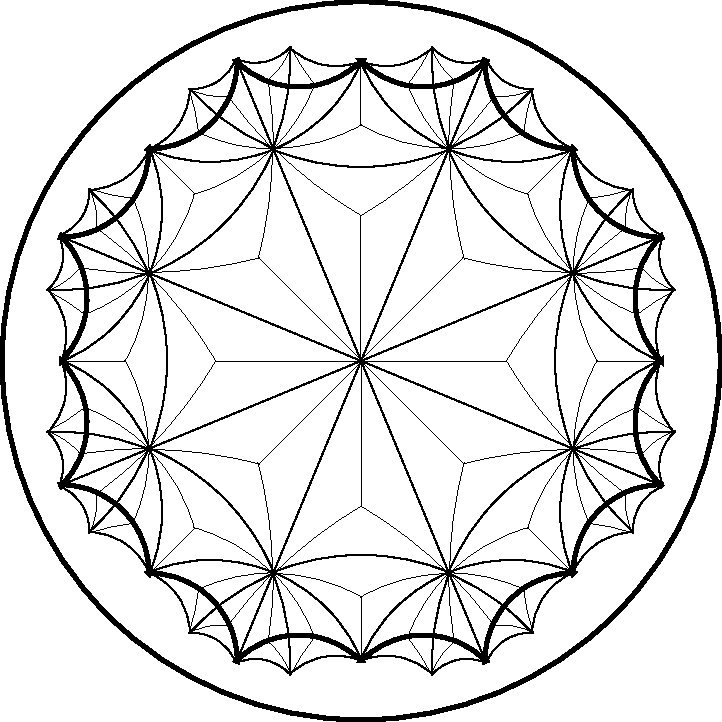
\includegraphics[width=1.3in]{figures/125_hyp_1.pdf}
\end{minipage}%
\begin{minipage}{.5\textwidth}
	\centering
	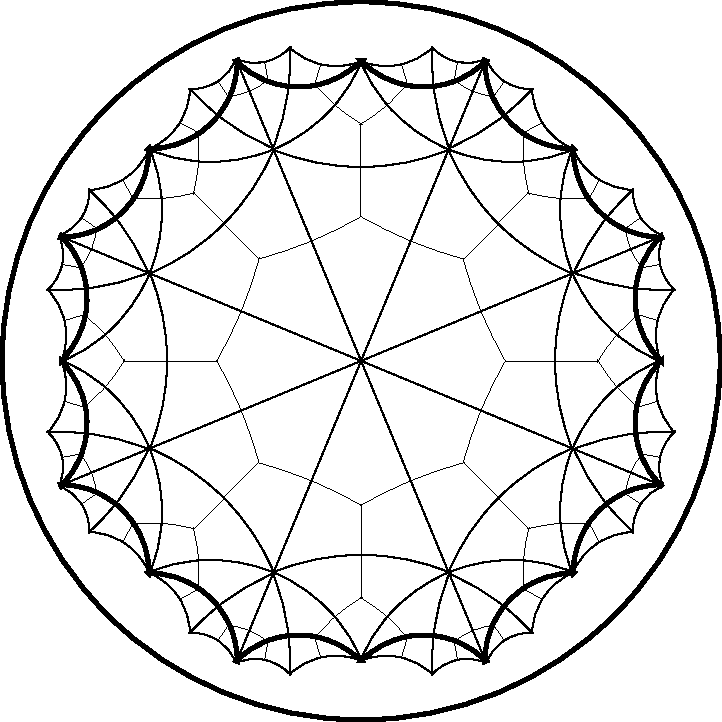
\includegraphics[width=1.3in]{figures/125_hyp_2.pdf}
\end{minipage}
\label{fig:125_hyp_i}
\end{figure}
\end{rem}


\begin{conjecture} \label{tessconj}
The output tessellation $\Delta_T$ of this algorithm always exists and $$\Aut(\Delta_T) \simeq \Aut(C)$$
\end{conjecture}


\subsubsection*{Tessellations on Octa-4}
We perform this algorithm to the underlying curve of Octa-4 as done in \cite{dami}. We begin with the base tessellation (Figure~\ref{fig:125}). The base tessellation of this curve is tiled by 24 regular hyperbolic $\frac{2 \pi}{8}$-triangles. Next, we locate all Weierstrass points. On $C,$ all vertices of the base tessellation correspond to Weierstrass points, that is $\Delta = \widetilde{\Delta}$. Each tile $T$ of $\widetilde{\Delta}$ is a regular triangle with all vertices the same weight, hence $G_T = D_3$. 

%We include an additional edge to mimic the $(2,3,7)$-tiling on Klein's quartic. This captures orientation-reversing automorphisms. Then, for the smallest tile $T',$ $T' \cup R(T')$ (where $R$ is a reflection about an edge) represents a fundamental domain for the action of $G_T$ on $T$ (Figure~\ref{fig:125_ref}). 

%%%lookd: if this is Z/3, why are there 6 tiles in T'
% this includes orientation-reversing ones. If it makes more sense, I will remove these lines.


%\footnote{For example, if the tile $T$ is a regular triangle with all 3 vertices the same weight, it has symmetry group $\Z/3$.}


%However, if not all Weierstrass points are located at the vertices of the base tessellation, we subdivide the tiles so that Weierstrass points are at the vertices.

%We claim that the smallest tile we achieve represents $\Aut(S).$

\begin{figure}[htbp] %  figure placement: here, top, bottom, or page
   \centering
   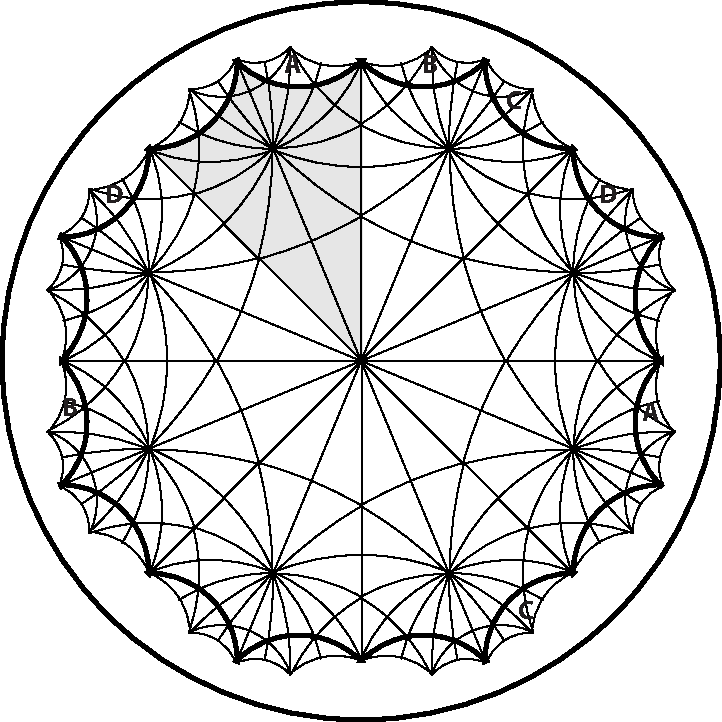
\includegraphics[width=2in]{figures/125_hyp} 
	\caption{The refined tessellation on $8(1, 2, 5)$}
	\label{fig:125_ref}
\end{figure}

%In general, we find all-seeing tessellations on such surfaces $S$ using prior knowledge of the automorphism group of $S$. 


%In some special cases, we know that our surface $S$ is in fact a quotient of a periodic polyhedral surface in $\R^3$, e.g. Fermat's curve, Schoen's I-WP Surface, and Bring's curve. In these very special cases, we can construct an all-seeing tessellation on $S$ without knowing the automorphism group of $S$ a priori. Thus, we can compute the automorphism group of $S$ from the all-seeing tessellation. \ti{prove that we can do it in the case of a quotient of a periodic polyhedral surface quotients?}

\section{Example Calculations}
\label{sec:examples}

This section is devoted to the computation of automorphism groups of our Riemann surfaces by all-seeing tessellations using the algorithm shown in section~\ref{sec:flagflag}. We checked the results programmatically with programs based on the algorithms of Bruin-Sijsling-Zotine \cite{jeroen}, which we discuss in section \ref{jeroen}.

As our test subjects, we consider a subset of examples from the classification of cyclic covers found in \cite{dthesis} that we expect to have large automorphism groups. 


%, we find an all-seeing tessellation and the associated automorphism group. 

%Then, we check this the correct automorphism group using the code described in section \ref{jeroen}.


 Table~\ref{table:plane} displays our results. The genus and (non)-hyperelliptic nature are calculated by tools from section~\ref{sec: dthesis}. 

\begin{table}[H]
\caption{Plane Curve Automorphism Groups}
\centering 
\begin{tabular}{ l | l c r r c} \hline
  \shortstack{Curve $C$} & Plane Curve Model & Genus & Aut($C$) & $|$Aut(C)$|$ \\ \hline
  $7(1, 2, 4)$ (Klein's quartic) & $y^3x + x^3 + 1$ & 3 & $GL_3(F_2)$ & 168 \\  % check if y^7 - x(x-1)^2 works, then let's switch to the latter
  $\ast 8(1, 1, 6)$ & $y^2 - (x^8 - 1)$  & 3 &  $D_4 \rtimes C_4$ & 32 \\ % check if y^8 - x(x-1)
  $8(1, 2, 5)$ (Fermat's quartic) & $y^4 - x (x+1) (x-1)$ & 3 & $C_4^{\text{ }2} \rtimes S_3$ & 96 \\ % y^8 - x(x-1)^2
  $\ast 12(1, 5, 6)$ &  $y^2 - (x^7 - x)$ & 3 & $C_4 \times S_3$ & 24 \\ % y^{12} - x(x-1)^5
  $5(1, 2, 4, 3)$ (Bring's curve) & $y^5 - x (x - 1)^2 (x + 1)^3$ & 4 & $S_5$ & 120 \\ 
  $12(1, 4, 7)$ (I-WP) & $y^3 - (x^5 - x)$ & 4 & $C_3 \times S_4$ & 72 \\ % y^{12} - x(x-1)^4
\end{tabular}
\label{table:plane} 
\caption*{An $\ast$ indicates that the curve is hyperelliptic}
\end{table}

%\begin{remark} Except f9, its automorphism group was calculated differently, and is discussed in its corresponding section. \end{remark}


In each of the following individual sections, we derive tessellations $\Delta_T$ to show that our examples satisfy Conjecture ~\ref{tessconj}.



\subsection*{7(1, 2, 4) Klein's quartic } 



Klein's quartic is a genus three curve that is a sevenfold cover over $\mathbb{C}\mathbb{P}^1$ with branching indices $(1,2,4)$ \cite{kw}. Its base tessellation is tiled by 56 triangles (Figure~\crefformat{figure}{~#2#1{(a)}#3} \cref{fig:124}). With the cone metric that arises from the branching indices and its multipliers, we get a basis of holomorphic 1-forms with the following divisors: $$(\omega_1) = \widetilde{p_2} + 3 \widetilde{p_3}, \qquad (\omega_2) = \widetilde{p_1} + 3 \widetilde{p_2}, \qquad (\omega_3) = 3 \widetilde{p_1} + \widetilde{p_3}.$$ All $\widetilde{p_i}$ are Weierstrass points with weight 1. Moreover, the \texttt{Resultant} of the wronski metric in \texttt{wronski.nb} tells us that the remaining Weierstrass points have weight one that arise from the midpoint of $\overline{p_i p_j}.$ We refine the tessellation with additional Weierstrass points as vertices and achieve the well-known tiling by $(\frac{\pi}{2}, \frac{\pi}{3}, \frac{\pi}{7})$-triangles (Figure~\crefformat{figure}{~#2#1{(b)}#3} \cref{fig:124}). Note that this tesellation exhibits orientation reversing automorphisms (reflections). 


\begin{figure}[htbp]
    \centering
    \subfloat[The base tessellation $\Delta$]{{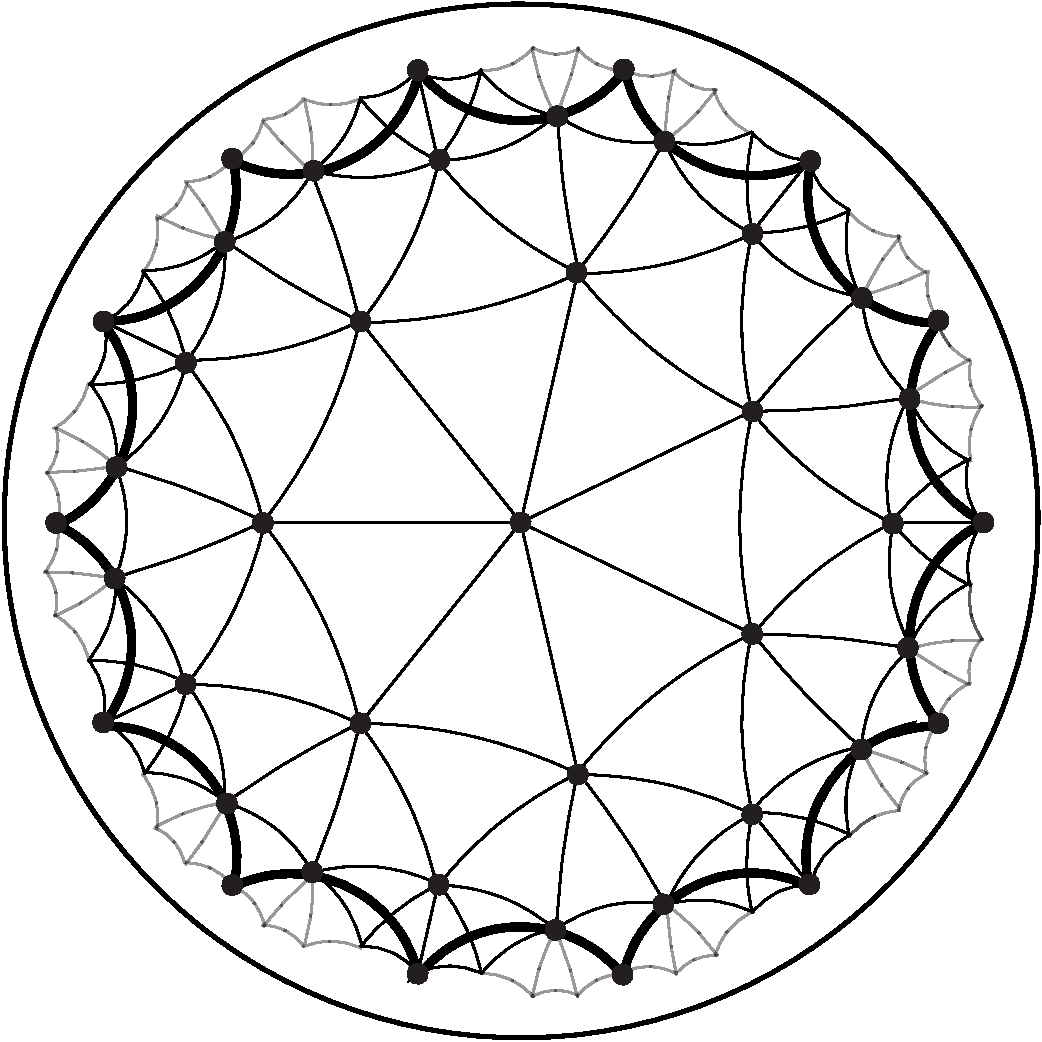
\includegraphics[width=2.75in]{figures/124_base_}}}
    \qquad
    \subfloat[The refined tessellation $\Delta_T$]{{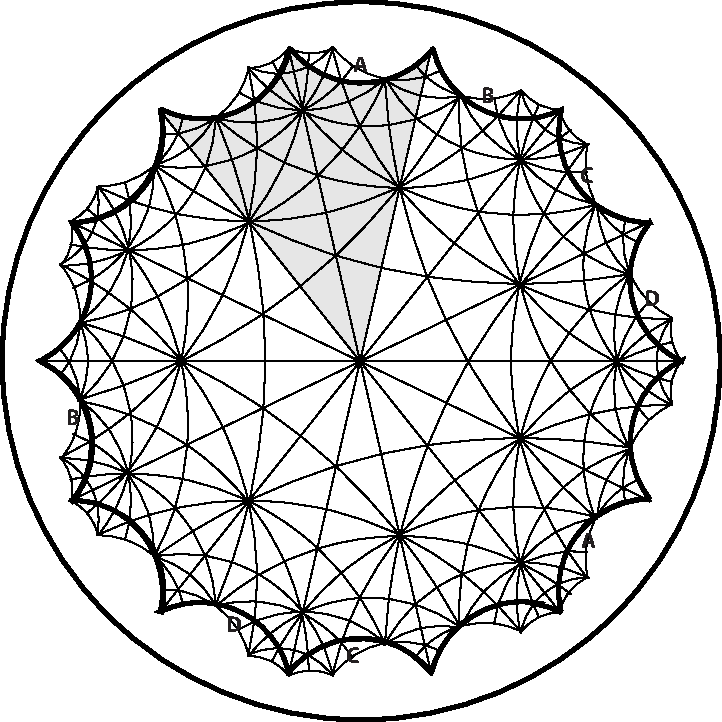
\includegraphics[width=2.75in]{figures/124_hyp_}}}%
    \caption{Klein's quartic}%
    \label{fig:124}%
\end{figure}

\subsection*{8(1, 1, 6)}
In this and the following subsection, we will look at two different hyperelliptic curves of genus three. First, we look at the eightfold cover defined by branching indices $(1, 1, 6).$ The branching indices along with the multipliers yield a basis of holomorphic 1-forms with divisors $$(\omega_1) = 4 \widetilde{p_3}, \qquad (\omega_2) = \widetilde{p_1} + \widetilde{p_2} + \widetilde{p_{3_1}} + \widetilde{p_{3_2}}, \qquad (\omega_3) = 2 \widetilde{p_1} + 2 \widetilde{p_2}.$$ Note that no $\widetilde{p_i}$ is a Weierstrass point. The wronski metric tells us that the Weierstrass points come from the midpoint of $\overline{p_1 p_2}.$ Hence we refine the tessellation to show all symmetries (Figure~\ref{fig:116}). These points are fixed under the hyperelliptic involution, whose quotient is a doubled octagon. In other words, we can rewrite the plane curve model as $y^2 - (x^8 - 1).$ 

\begin{figure}[htbp]
    \centering
    \subfloat{{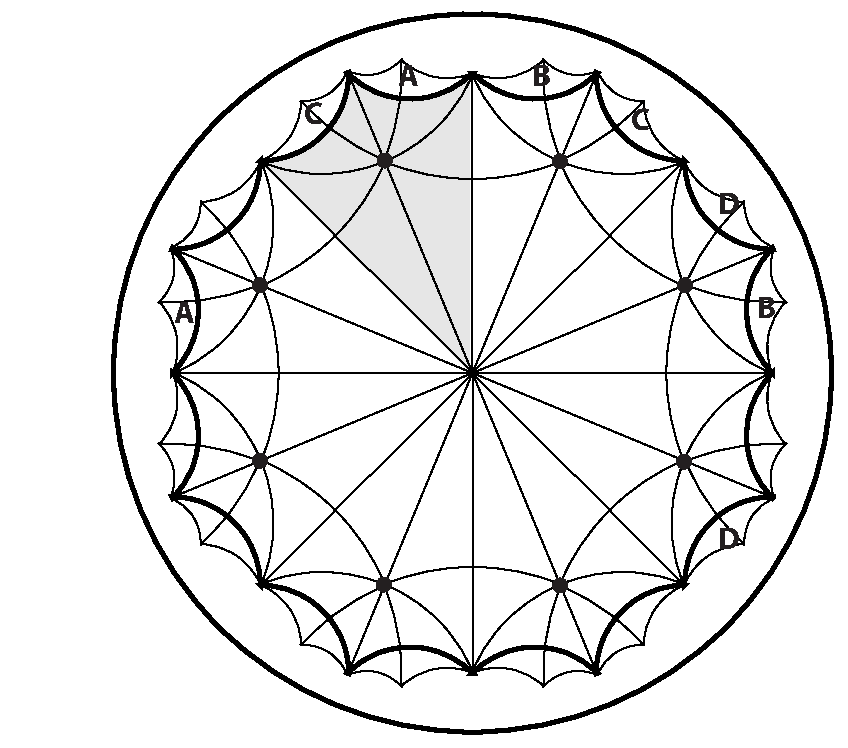
\includegraphics[width=2.75in]{figures/116_hyp}}}
    \caption{Hyperbolic tessellation on $8(1, 1, 6)$}%
    \label{fig:116}%
\end{figure}




\subsection*{12(1, 5, 6)}
%f10
This curve is another genus three hyperelliptic curve that is defined as a twelvefold cover over a sphere with branching indices $(1, 5, 6).$ We achieve a basis of 1-forms with divisors $$(\omega_1) = 4 \widetilde{p_2}, \qquad (\omega_2) = 2 \widetilde{p_1} + 2 \widetilde{p_2}, \qquad (\omega_3) = 4 \widetilde{p_2},$$ hence $\widetilde{p_1}$ and $\widetilde{p_2}$ are Weierstrass points of weight 3 each. Recall that if $q$ for $q \neq p_i$ is a zero of the Wronski metric, then there must be 12 preimages $\widetilde{q}$ on the genus three curve, which contradicts the total weight theorem ($g^3 - g$). However, the wronski metric tells us that $p_3$ is in fact a triple order zero, hence all six $\widetilde{p_{3_i}}$ are Weierstrass points. All Weierstrass points are marked as either $\bullet$ or $\circ$ as they have different valency (Figure~\ref{fig:156}). The surface is a double cover over a Riemann sphere branched at six points which are located at the North and South Pole, and six equidistributed points on the Equator. Hence, the plane curve model can also be written as $y^2 - (x^7 - x).$

\begin{figure}[htbp]
    \centering
    \subfloat{{\includegraphics[width=2.75in]{figures/156_hyp_}}}
    \caption{Hyperbolic tessellation on $12(1, 5, 6)$}%
    \label{fig:156}%
\end{figure}




%$X_{(156)}$ is a twelvefold cover with branching indices $12(1, 5, 6)$,

%\begin{lemma} X10 is hyperelliptic and of genus three. \end{lemma}


%It is infact https://groupprops.subwiki.org/wiki/Nontrivial_semidirect_product_of_Z3_and_Z8 

%\begin{remark} In particular, $Aut(J, a)$ is a semidirect product $C_2 \rtimes C_{12}$ ($C_2$ is normal), and the action $C_2 \to Aut(C_{12})$ sends $g \mapsto gmg^{-1} = m^5$. It is not obviously the usual dihedral or dicyclic group.\end{remark}



% On its tessellation (Figure~\crefformat{figure}{~#2#1{(a)}#3} \cref{fig:156}), all vertices are Weiertrass points of equal weight. However, by identification of edges, one can see that not all vertices are similar. At the center of the tessellation is 12-valent but not all vertices are. Hence, we denote them with different markings. Then by the same argument as in $6(1, 1, 4),$ $12(1, 3, 8),$ and $8(1, 1, 6),$ $|\Aut|$ equals the number of triangles that appear on the tessellation.


\subsection*{12(1, 4, 7) Schoen's I-WP Surface}

%f6 

In this section, we look at another genus four non-hyperelliptic curve. This curve appears in \cite{dthesis} as the underlying curve of a triply periodic polyhedral surface called Octa-8. The fundamental piece of the polyhedral surface is tiled by 24 triangles which appear in Figure~\crefformat{figure}{~#2#1{(a)}#3} \cref{fig:147}. The curve is a twelvefold cover over $\mathbb{C}\mathbb{P}^1$ with branching indices $(1, 4, 7).$ By admissible cone metrics, we obtain a basis of 1-forms with divisors $$(\omega_1) = 6 \widetilde{p_3}, \qquad (\omega_2) = \widetilde{p_1} + \widetilde{p_{2_1}} + \widetilde{p_{2_2}} + \widetilde{p_{2_3}} + \widetilde{p_{2_4}} + \widetilde{p_3}, \qquad (\omega_3) = 2 \widetilde{p_1} + 2 \widetilde{p_3}, \qquad (\omega_4) = 6 \widetilde{p_1}.$$

The wronski metric tells us that three simple zeros are located at the midpoint of $\overline{p_i p_j}$ for all $i$ and $j.$ We obtain a refined tessellation (Figure~\crefformat{figure}{~#2#1{(b)}#3} \cref{fig:147}) where vertices marked as $\bullet$ have weight four, and those marked as $\circ$ have weight one. 



\begin{figure}[htbp]
    \centering
    \subfloat[The base tessellation $\Delta$]{{\includegraphics[width=2.75in]{figures/147_base_}}}
    \qquad
    \subfloat[The refined tessellation $\Delta_T$]{{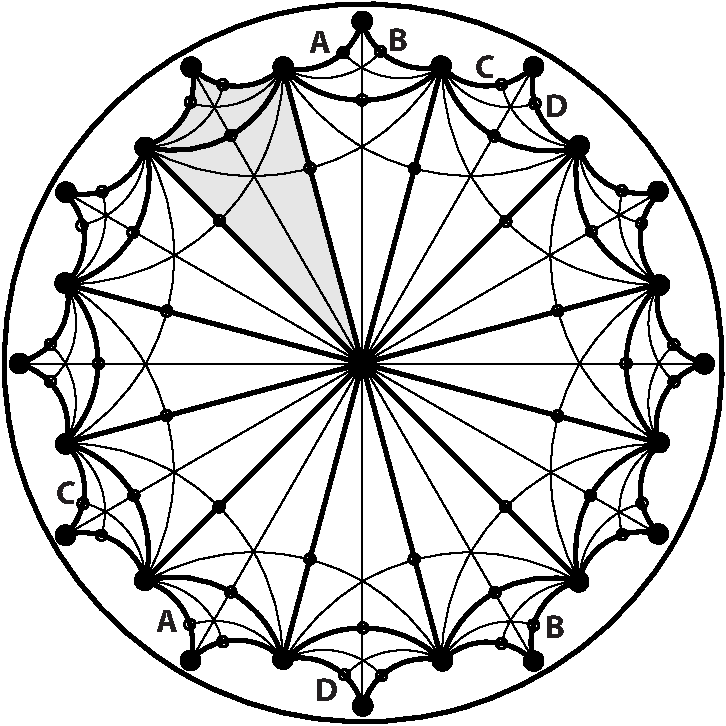
\includegraphics[width=2.75in]{figures/147_weight_}}}%
    \caption{12(1,4,7)}%
    \label{fig:147}%
\end{figure}


\section{Programmatic Method of Checking Conjecture}

We checked our calculations of an all-seeing tessellation of a curve $C$ by taking a plane curve presentation of $C$, and plugging into our program \texttt{autplane.sage} based on the algorithms of Bruin-Sijsling-Zotine (Section 4.1, \cite{jeroen}). Our code is available at \begin{center} \texttt{https://github.com/catherineray/aut-jac/autplane.sage} \end{center}.

\begin{remark}We exposit the algebreo-geometric and programmatic background of this section in much more detail in our sequel paper \textit{The Study of Principal Polarizations through Automorphisms of the Jacobian}.\end{remark}

The brilliance of Bruin-Sijsling-Zotine's approach is proving that given plane algebraic curves (not necessarily smooth) and their Jacobians, we may \textit{heuristically} calculate their automorphisms, and obtain rigorous results. 





%\begin{remark} Note that the University of Bristol's GroupNames database at the time of writing has groups up to order 500 with full names and structure description. In the cases where the order is greater than 500, we use the output of \texttt{StructureDescription(G);}  \end{remark}

%Considering the orientation of each triangles, we see that we can not choose any two triangles in the tessellation. However, the tessellation can be divided into two congruence classes of 72 triangles each. Given two triangles from the same congruence class, there is one map that maps one triangle to the other. As in $12(1, 3, 8)$ we saw earlier, the weights of the vertices must be preserved. Hence, $|\Aut(\text{I-WP})| = 72.$




%\begin{thm*} $X6$ is nonhyperelliptic and of genus 4. It is shown in the thesis of the first author \cite{dthesis} that this is the Schoen I-WP Surface. \end{thm*} 

%https://ntrs.nasa.gov/archive/nasa/casi.ntrs.nasa.gov/19700020472.pdf


% We present the intersection matrix used to make the period matrix, note it shows that the surface is cyclic.




\begin{thebibliography}{20}


\bibitem{jeroen}
N. Bruin, J. Sijsling, A. Zotine,
\textit{Numerical Computation of Endomorphism Rings of Jacobians},
The Open Book Series,
Vol. 2, 2019, pp. 155--171, Mathematical Sciences Publishers.

\bibitem{fk}
H. Farkas, I. Kra,
\textit{Riemann Surfaces},
Springer-Verlag, New York, 1992.

\bibitem{kw}
H. Karcher, M. Weber,
\textit{On Klein's Riemann Surface},
The Eightfold Way, MSRI Publications, 
Vol. 35, 1998, pp.9--49.

\bibitem{sl}
Z. Laing, D. Singerman,
\textit{Transitivity on Weierstrass Points}
Annales Academiae Scientiarum Fennicae Mathematica,
Vol. 37, 2012, pp.285--300

\bibitem{dami} 
D. Lee,
\textit{On a triply periodic polyhedral surface whose vertices are Weierstrass points},
Arnold Mathematical Journal, 
Vol. 3, Issue 3, 2017, pp.319--331.

\bibitem{dthesis} 
D. Lee, 
\textit{Geometric realizations of cyclically branched coverings over punctured spheres},
\texttt{https://arxiv.org/abs/1809.06321}, preprint.

\bibitem{hyp}
R. Lercier, C. Ritzenthaler, J. Sijsling,
\textit{Fast computation of isomorphisms of hyperelliptic curves and explicit Galois descent},
Proceedings of the Tenth Algorithmic Number Theory Symposium, Mathematical Sciences Publishers.,
2013, pp. 463–-486.

\bibitem{silverman}
J. H. Silverman,
\textit{The Arithmetic of Elliptic Curves},
Springer-Verlag, New York, 2009.

\bibitem{matti} 
M. Weber,
\textit{Kepler's small stellated dodecahedron as a Riemann surface},
Pacific Journal of Mathematics, 
Vol. 220, 2005, pp.167--182.


\end{thebibliography}
\end{document}
